\bookchapter{Capitolo 42: Panorama dei modelli di grandi dimensioni e pratica con le API}

\chapterintro{I capitoli precedenti hanno parlato di “come collaborare con l'AI”; questo capitolo risolve una questione più fondamentale: “quale AI usare? E come?”. Nel panorama di agosto 2026 i modelli di grandi dimensioni sono ricchissimi — a livello internazionale si contendono il primato GPT, Claude e Gemini, mentre in Cina fioriscono DeepSeek, Tongyi Qianwen, GLM, Kimi e Doubao. Ogni modello ha il suo carattere e i suoi punti di forza: la scelta giusta raddoppia i risultati con metà dello sforzo, quella sbagliata fa l'opposto. Questo capitolo non ti fa solo conoscere questi modelli, ma ti insegna anche come collegarli alle tue applicazioni tramite API e come scegliere il Token Plan (il piano d'uso) giusto in base alle tue necessità.}

\booksection{I modelli internazionali principali: il dominio dei tre grandi}

Nel mercato internazionale dei modelli di grandi dimensioni di agosto 2026 si è consolidato un equilibrio a tre: OpenAI (serie GPT), Anthropic (serie Claude) e Google (serie Gemini). Ognuno ha una personalità ben marcata — facciamo conoscenza uno per uno.

\booksubsection{La serie OpenAI GPT-5.6: l'atleta completo ed equilibrato}

OpenAI ha dato il via all'ondata dei modelli di grandi dimensioni e la serie GPT resta ancora oggi il modello più usato al mondo. La serie GPT-5.6, rilasciata a luglio 2026, adotta una strategia a tre livelli: il flagship GPT-5.6 Sol punta alle esigenze di ragionamento di alto livello, l'equilibrato GPT-5.6 Terra allo sviluppo quotidiano, il leggero GPT-5.6 Luna agli scenari ad alta concorrenza e basso costo. I tre modelli condividono una finestra di contesto di 1,05 milioni di Token e supportano tutti input di immagini, function calling e output strutturato.

\begin{center}
\begin{tabularx}{\linewidth}{|X|X|X|X|X|}
\hline
\textbf{Modello} & \textbf{Posizionamento} & \textbf{Input (/milione di Token)} & \textbf{Output (/milione di Token)} & \textbf{Finestra di contesto} \tabularnewline
\hline
GPT-5.6 Sol & Flagship per il ragionamento & 5,00 USD (circa 36 yuan) & 30,00 USD (circa 217 yuan) & 1,05 milioni di Token \tabularnewline
GPT-5.6 Terra & Equilibrato per l'uso quotidiano & 2,50 USD (circa 18 yuan) & 15,00 USD (circa 109 yuan) & 1,05 milioni di Token \tabularnewline
GPT-5.6 Luna & Leggero e a basso costo & 1,00 USD (circa 7 yuan) & 6,00 USD (circa 44 yuan) & 1,05 milioni di Token \tabularnewline
\hline
\end{tabularx}
\end{center}

\begin{center}\small\color{gray}Prezzi della serie OpenAI GPT-5.6 (agosto 2026)\end{center}

Il vantaggio principale della serie GPT è l'equilibrio — ragionamento, programmazione, scrittura, multimodalità: nessun vero punto debole. In più, l'ampio ecosistema di plugin e la community di sviluppatori di OpenAI offrono la documentazione di adattamento e la toolchain più complete. Negli scenari in cui “non sai cosa scegliere”, GPT è la risposta predefinita che “non sbagli nemmeno a occhi chiusi”. Ma i suoi limiti sono: per accedervi dalla Cina serve una rete particolare, l'espressione in cinese ogni tanto ha un “sapore di traduzione” e i prezzi delle API si collocano su livelli medio-alti.

\textbf{Buone notizie}\par

Nell'agosto 2026 OpenAI ha annunciato che il modello predefinito per gli utenti gratuiti diventa GPT-5.6 Luna, con chat testuale illimitata. Significa che puoi sperimentare le capacità di base di GPT a costo zero, pagando solo se ti serve un ragionamento più potente o le chiamate API.

\booksubsection{La serie Anthropic Claude: il vertice della programmazione e del rigore}

Se GPT è l'atleta completo, Claude è il “tetto” nel campo della programmazione. La serie Claude di Anthropic guida da tempo con margine netto nella SWE-bench (benchmark di ingegneria del software), prima al mondo per qualità della generazione di codice e capacità di realizzare progetti a livello ingegneristico. Ancora più raro: il tasso di allucinazioni di Claude (la probabilità di generare informazioni false) è il più basso in assoluto, circa l'1\% — il che lo rende particolarmente adatto a scenari di alta precisione come l'accademico e il legale.

L'altro asso nella manica di Claude è il contesto ultralungo: una finestra di contesto da 1 milione di Token che gli permette di “leggere d'un fiato” centinaia di pagine di contratti o un'intera base di codice senza perdere dettagli. Nel refactoring del codice e nell'analisi di documenti lunghi è praticamente insostituibile. Claude Code, come strumento di programmazione AI da terminale, ha raggiunto a metà 2026 un fatturato annualizzato di 2,5 miliardi di dollari — la prova più evidente di quanto le capacità di programmazione di Claude siano apprezzate.

\begin{center}
\begin{tabularx}{\linewidth}{|X|X|X|X|X|}
\hline
\textbf{Modello} & \textbf{Posizionamento} & \textbf{Input (/milione di Token)} & \textbf{Output (/milione di Token)} & \textbf{Finestra di contesto} \tabularnewline
\hline
Claude Fable 5 & Versione flagship & 10,00 USD (circa 72 yuan) & 50,00 USD (circa 362 yuan) & 1 milione di Token \tabularnewline
Claude Opus 4.8 & Versione professionale & 5,00 USD (circa 36 yuan) & 25,00 USD (circa 181 yuan) & 1 milione di Token \tabularnewline
Claude Sonnet 5 & Versione economico-efficiente & 2,00 USD (circa 14 yuan) & 10,00 USD (circa 72 yuan) & 1 milione di Token \tabularnewline
\hline
\end{tabularx}
\end{center}

\begin{center}\small\color{gray}Prezzi della serie Anthropic Claude (agosto 2026; Sonnet 5 a prezzo promozionale)\end{center}

Il punto debole di Claude è il prezzo: l'output di Fable 5 è il più caro tra tutti i modelli, 50 dollari per milione di Token. Anche le capacità multimodali (comprensione di immagini e video) sono relativamente deboli. Per gli sviluppatori individuali con budget limitato, Sonnet 5 nel periodo promozionale ha un rapporto qualità-prezzo davvero notevole.

\booksubsection{La serie Google Gemini: il re della multimodalità}

La serie Gemini di Google nel 2026 è arrivata alla versione 3.1 Pro. L'asso principale di Gemini è la multimodalità nativa — analisi precisa di testo e immagini, riconoscimento OCR delle tabelle senza errori, estrazione efficiente dei fotogrammi video, oltre all'analisi approfondita di audio e video. È legato a fondo all'ecosistema Google (ricerca, email, servizi cloud) e si distingue nel recupero di informazioni in tempo reale e nella comprensione cross-modale. Gemini supporta anche input di contesto ultralungo da 2 milioni di Token ed è attualmente il modello con la finestra di contesto più grande.

Gemini si posiziona come “prima scelta per il ragionamento scientifico e gli scenari multimodali”. Se il tuo progetto coinvolge molte analisi di immagini, comprensione di video o calcolo scientifico, Gemini non ha praticamente rivali. Però nella generazione di codice puramente testuale è un po' sotto Claude, e l'espressione in cinese è meno naturale di quella dei modelli nazionali.

\begin{center}
\begin{tabularx}{\linewidth}{|X|X|X|X|}
\hline
\textbf{Elemento di confronto} & \textbf{GPT-5.6} & \textbf{Claude Fable 5} & \textbf{Gemini 3.1 Pro} \tabularnewline
\hline
Punteggio complessivo & 94.8 & 95.0 & 92.1 \tabularnewline
Capacità di programmazione (SWE-bench) & 74.9\% & 64.3\% (Pro) & Media \tabularnewline
Finestra di contesto & 1,05 milioni di Token & 1 milione di Token & 2 milioni di Token \tabularnewline
Capacità multimodali & Equilibrate & Deboli & Le più forti \tabularnewline
Tasso di allucinazioni & Basso & Il più basso (circa 1\%) & Basso \tabularnewline
Disponibilità in Cina & Richiede rete particolare & Richiede rete particolare & Richiede rete particolare \tabularnewline
Ecosistema API & Il più completo & In crescita & Legato all'ecosistema Google \tabularnewline
\hline
\end{tabularx}
\end{center}

\begin{center}\small\color{gray}Confronto orizzontale dei tre grandi modelli internazionali (agosto 2026)\end{center}

\begin{tcbwarn}{Nota: l'ostacolo concreto dell'uso dalla Cina}
Per gli sviluppatori in Cina, l'ostacolo principale di GPT, Claude e Gemini è l'accesso alla rete. Pur potendoli usare indirettamente tramite proxy Azure o piattaforme di aggregazione API, stabilità e conformità vanno valutate in autonomia. Se il tuo progetto ha requisiti severi di sicurezza dei dati, ti consiglio di dare priorità ai modelli nazionali.

\end{tcbwarn}

\booksection{I principali modelli nazionali: una fioritura di proposte}

Nel 2026 i modelli nazionali sono passati da “inseguitori” a “concorrenti alla pari”, e in certi ambiti hanno persino preso il comando. A differenza delle controversie sul “restyling” del 2023, i modelli flagship nazionali del 2026 hanno raggiunto i modelli internazionali di prima fascia nel ragionamento logico, nella generazione di codice e nella comprensione del cinese, riducendo il divario sotto il 5\%. Ancora più importante: i modelli nazionali hanno vantaggi insostituibili negli scenari in cinese, nei costi e nel deployment conforme.

\booksubsection{DeepSeek V4: il re del rapporto qualità-prezzo}

DeepSeek è un fenomeno tra i modelli nazionali. All'inizio del 2025, DeepSeek-V3 ha scosso il mercato posizionandosi come “un decimo del costo di GPT con capacità equivalenti”, tanto che nel settore è stato definito la “soglia fatale dei modelli AI generalisti” — i più economici di lui non sono altrettanto validi, i più costosi non offrono lo stesso volume. Ad agosto 2026 è arrivata la versione ufficiale di DeepSeek V4-Pro: architettura MoE da 1,6 mila miliardi di parametri con circa 49B attivati, supporto per 1 milione di Token di contesto senza degrado, e un rapporto qualità-prezzo nel codice ampiamente considerato il migliore al mondo.

DeepSeek V4 ha fatto un grande salto nelle capacità Agent — il benchmark DeepSWE è passato da 12.8 a 62.7 (+390\%) e NL2Repo da 38.5 a 61.5. Le API aggiungono il doppio protocollo Responses API e Anthropic API, già compatibili con gli strumenti di programmazione principali come Codex e Claude Code. Significa che puoi sostituire le API di Claude con quelle di DeepSeek dentro Claude Code — costi ridotti di diverse volte con un'esperienza quasi identica.

\begin{center}
\begin{tabularx}{\linewidth}{|X|X|X|X|X|}
\hline
\textbf{Modello} & \textbf{Posizionamento} & \textbf{Input (/milione di Token)} & \textbf{Output (/milione di Token)} & \textbf{Finestra di contesto} \tabularnewline
\hline
DeepSeek V4 Pro & Flagship per il ragionamento & 3 yuan (circa 0,43 USD) & 6 yuan (circa 0,87 USD) & 1 milione di Token \tabularnewline
DeepSeek V4 Flash & Leggero e veloce & 1 yuan (circa 0,14 USD) & 2 yuan (circa 0,28 USD) & 1 milione di Token \tabularnewline
\hline
\end{tabularx}
\end{center}

\begin{center}\small\color{gray}Prezzi della serie DeepSeek V4 (agosto 2026, prezzi promozionali)\end{center}

Confronto di prezzo: per 1 milione di Token di input + 1 milione di Token di output, DeepSeek V4 Flash costa circa 0,42 dollari, GPT-5.6 Sol circa 35 dollari e Claude Fable 5 circa 60 dollari. Un divario fino a 80-140 volte.

\textbf{Avviso per evitare trappole: DeepSeek sta per aumentare i prezzi}\par

DeepSeek ha comunicato ufficialmente il 6 agosto 2026 di “prevedere a breve un forte aumento dei prezzi delle API”, quindi i prezzi promozionali potrebbero non durare ancora a lungo. Alcuni media parlano di aumenti fino a 30 volte, ma al 14 agosto l'ufficialità non ha ancora pubblicato il piano di adeguamento definitivo. Inoltre DeepSeek V4 nella versione ufficiale introduce una tariffazione differenziata per fasce orarie — nelle ore di punta il costo delle chiamate raddoppia in pieno. Ti consiglio di seguire gli annunci ufficiali per i prezzi aggiornati.

\booksubsection{Tongyi Qianwen Qwen3.7 Max: la scelta enterprise di Alibaba Cloud}

La serie Tongyi Qianwen (Qwen) di Alibaba Cloud poggia sull'ecosistema Alibaba Cloud e ha un vantaggio naturale nel deployment enterprise. Qwen3.7 Max di luglio 2026 è l'attuale flagship: modello denso da 235B di parametri con contesto nativo di 256K, estendibile a 1M. I vantaggi principali di Qwen: un ecosistema open source maturo (tutta la serie da 7B a 235B è open source), una comprensione precisa degli scenari in cinese e un'integrazione profonda con l'infrastruttura Alibaba Cloud.

\begin{center}
\begin{tabularx}{\linewidth}{|X|X|X|}
\hline
\textbf{Modello} & \textbf{Prezzo output (/milione di Token)} & \textbf{Scenari d'uso} \tabularnewline
\hline
qwen-turbo & 0,6 yuan & Domande e risposte essenziali, classificazione del testo, alta concorrenza \tabularnewline
qwen-long & 2,0 yuan & Elaborazione di contesti ultralunghi da 10M \tabularnewline
qwen3.7-flash & 7,2 yuan & Conversazione generale, generazione di contenuti \tabularnewline
qwen3.7-plus & 12,0 yuan & Multimodale (immagini + video), creazione in cinese \tabularnewline
qwen3.7-max & 36,0 yuan & Capacità cinese di punta, compiti complessi \tabularnewline
\hline
\end{tabularx}
\end{center}

\begin{center}\small\color{gray}Prezzi a scaglioni della serie Tongyi Qianwen Qwen (agosto 2026)\end{center}

I prezzi di Qwen seguono una strategia a scaglioni — dal qwen-turbo a costo minimo (output 0,6 yuan per milione di Token) al flagship qwen3.7-max (output 36 yuan per milione di Token), coprendo tutto, dalle domande e risposte leggere al ragionamento complesso. Per le aziende che già usano Alibaba Cloud, Qwen è la scelta di integrazione più comoda.

\booksubsection{GLM-5.1 di Zhipu: primo posto nazionale nella SWE-bench}

La serie GLM di Zhipu AI nel 2026 brilla. GLM-5.1 conquista il primo posto nazionale nella SWE-bench: architettura ibrida MoE/densa da 744B, con supporto per 1 milione di Token di contesto. Si distingue per la comprensione semantica precisa del cinese e supporta il deployment privato conforme alle regole nazionali — fondamentale per finanza e pubblica amministrazione, dove i requisiti di sicurezza dei dati sono elevati. I prezzi di GLM-5.1 sono 6 yuan di input e 24 yuan di output per milione di Token, nella fascia intermedia dei modelli nazionali.

\booksubsection{Kimi K3: il re dei testi ultralunghi}

La serie Kimi di Moonshot AI è celebre per la capacità di elaborare testi ultralunghi. Kimi K3, rilasciato a luglio 2026, scala 2,8 mila miliardi di parametri ed entra nella prima fascia mondiale in molte valutazioni su compiti complessi. Lo scenario principale di Kimi è l'analisi di basi di codice lunghe e il recupero potenziato su documenti lunghi — sa gestire il testo di un libro intero o il codice di un intero progetto ed eccelle nelle ricerche tipo “ago nel pagliaio”. I prezzi di Kimi sono relativamente alti (output circa 12-20 yuan per milione di Token), ma nel rapporto qualità-prezzo sui testi lunghi nessuno fa meglio.

\booksubsection{Doubao: l'atleta completo di ByteDance}

La serie Doubao di ByteDance nel 2026 si conferma stabile. Doubao Seed 2.1 Pro è il modello flagship di Volcano Engine, con contesto da 256K, prestazioni complessive stabili nelle prove pratiche e un'esperienza eccellente negli scenari in cinese. I vantaggi di Doubao: alla registrazione regala molti Token gratuiti, l'integrazione con l'ecosistema Volcano Engine è completa e i prezzi sono tra i più bassi in Cina. Per i principianti che vogliono provare subito la programmazione AI, Doubao è la scelta d'ingresso a barriera zero.

\begin{center}
\begin{tabularx}{\linewidth}{|X|X|X|X|X|X|}
\hline
\textbf{Elemento di confronto} & \textbf{DeepSeek V4} & \textbf{Qwen3.7 Max} & \textbf{GLM-5.1} & \textbf{Kimi K3} & \textbf{Doubao 2.1 Pro} \tabularnewline
\hline
Punteggio complessivo & 87.5 & 89.7 & 90.5 & 88+ & 85+ \tabularnewline
Capacità di programmazione & Fortissima & Forte & Primo SWE nazionale & Forte & Medio-alto \tabularnewline
Comprensione del cinese & Ottima & Ottima & Precisa & Ottima & Ottima \tabularnewline
Finestra di contesto & 1 milione & 256K-1M & 1 milione & Ultralunga & 256K \tabularnewline
Prezzo output (yuan/M) & 6 & 36 & 24 & 12-20 & 30 \tabularnewline
Open source & Licenza MIT & Tutta la serie open source & Parzialmente open source & Closed source & Closed source \tabularnewline
Deployment privato & Supportato & Supportato & Supportato & Non supportato & Non supportato \tabularnewline
\hline
\end{tabularx}
\end{center}

\begin{center}\small\color{gray}Confronto orizzontale dei cinque grandi modelli nazionali (agosto 2026)\end{center}

Una tendenza importante: il “divario generazionale” percepito tra i modelli nazionali e GPT/Claude è sparito. Nel ragionamento logico e nelle competizioni matematiche la differenza tra i flagship nazionali e GPT-5 è ormai di una cifra. Nel pensiero architetturale sistematico e nel ragionamento d'ingegneria complessa Claude resta in vantaggio — propone soluzioni architetturali più “ispirate”, mentre i modelli nazionali a volte appaiono “dogmatici”. Ma negli scenari in cinese, nel controllo dei costi e nel deployment conforme, i modelli nazionali hanno un vantaggio schiacciante.

\begin{center}
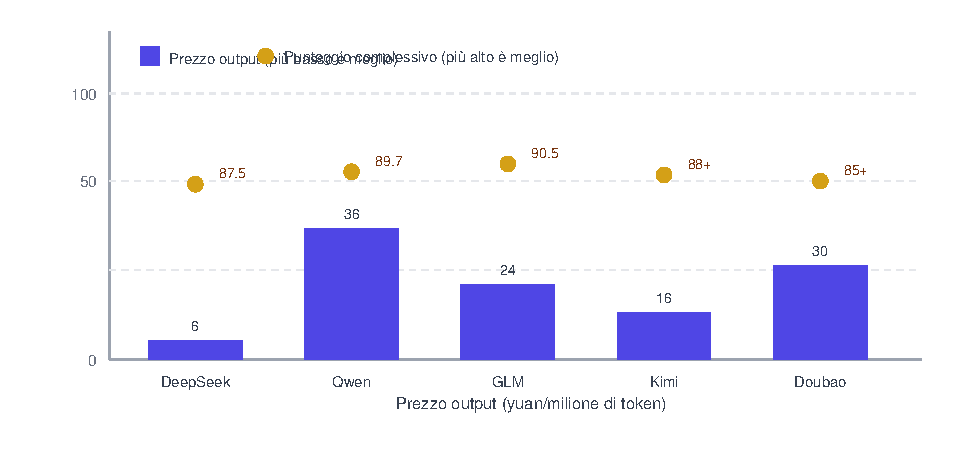
\includegraphics[width=0.92\linewidth]{figures/fig-di-si-shi-er-zhang-1}
\\[2pt]\small Figura 4: confronto di prezzo e prestazioni tra i cinque modelli (prezzo più basso è meglio, punteggio più alto è meglio)
\end{center}

\booksection{Quadro decisionale per la scelta del modello}

Conosciute le caratteristiche di ogni modello, come scegliere quello per il tuo progetto? Ecco il “metodo decisionale delle quattro domande”: rispondi a quattro domande e individuerai il modello più adatto a te.

Il progetto viene distribuito in Cina o a livello internazionale?

Cina scegli un modello cinese

|

Internazionale vali anche i modelli esteri

Il compito principale è programmare o altro?

Codice Claude o DeepSeek

|

Altro continua a decidere

Serve un contesto extra-lungo (>500 mila token)?

Sì Gemini o Kimi

|

No continua a decidere

Il budget è un vincolo?

Sì DeepSeek o Qwen-turbo

|

No GPT-5.6 o Claude

\begin{center}\small\color{gray}Figura 5: il metodo decisionale delle quattro domande per scegliere il modello\end{center}

\begin{tcbinfo}{Suggerimento: strategia combinata}
Questo metodo non è un dogma — in molti scenari serve combinare più modelli. Una strategia combinata comune: DeepSeek o Qwen per lo sviluppo quotidiano (costi bassi, cinese ottimo), Claude per il design architetturale critico (ragionamento forte, poche allucinazioni), Gemini per l'analisi multimodale (elaborazione di immagini e video). Cambia modello secondo il bisogno invece di “usarne uno per tutta la vita”.

\end{tcbinfo}

\booksection{Introduzione alle chiamate API: collegare i modelli partendo da zero}

Molti tutorial di programmazione AI insegnano solo a usare l'interfaccia di chat, ma la vera “programmazione AI” — far sì che la tua applicazione chiami i modelli di grandi dimensioni — passa dalle API. Le API (Application Programming Interface, interfacce di programmazione delle applicazioni) sono protocolli di comunicazione tra programmi. Tramite API, il tuo codice può invocare le capacità del modello come se chiamasse una funzione.

\booksubsection{Cos'è un Token}

Prima di capire le API devi comprendere il concetto di “Token”. Il Token è l'unità base di fatturazione dei modelli di grandi dimensioni: puoi vederlo come “l'unità di lettura e scrittura dell'AI”. Un Token corrisponde all'incirca a 0,75 parole inglesi (4 caratteri) oppure a 0,5-1 carattere cinese. Un testo cinese di 1000 caratteri consuma circa 1500-2000 Token.

I Token non sono parole, né caratteri. I modelli di grandi dimensioni usano un tokenizer dedicato per dividere il testo in Token. La stessa parola può contare Token diversi nei vari modelli — per esempio, la parola “intelligenza artificiale” può valere 3 Token in GPT e 2 in DeepSeek. Le API della maggior parte dei modelli restituiscono il numero di Token effettivamente consumato, che puoi vedere nella risposta API.

\begin{tcbinfo}{Stima rapida dei costi in Token}
1 milione di caratteri cinesi equivalgono a circa 1,5 milioni di Token. Con DeepSeek V4 Flash, elaborare 1 milione di caratteri di input + 1 milione di output costa circa 0,42 dollari (circa 3 yuan); con Claude Fable 5 la stessa quantità costa circa 60 dollari (circa 434 yuan). Ecco perché la scelta del modello incide direttamente sul costo del tuo progetto.

\end{tcbinfo}

\booksubsection{Ottenere una API Key}

Il primo passo per usare le API dei modelli di grandi dimensioni è ottenere una API Key — una sequenza di caratteri usata per l'autenticazione. Ogni fornitore di modelli ha la sua piattaforma API: devi registrare un account e creare la API Key. Ecco gli ingressi delle piattaforme API dei modelli principali e le procedure per ottenerla:

\begin{center}
\begin{tabularx}{\linewidth}{|X|X|X|X|}
\hline
\textbf{Modello} & \textbf{Piattaforma API} & \textbf{Procedura di ottenimento} & \textbf{Quota gratuita} \tabularnewline
\hline
DeepSeek & platform.deepseek.com & Registrazione verifica dell'identità creazione della API Key & Quota in omaggio per i nuovi utenti \tabularnewline
Tongyi Qianwen & bailian.aliyun.com (piattaforma Bailian) & Accesso con account Alibaba Cloud attivazione del servizio creazione della Key & Prova gratuita per i nuovi utenti \tabularnewline
Zhipu GLM & open.bigmodel.cn & Registrazione verifica dell'identità creazione della API Key & Quota in omaggio per i nuovi utenti \tabularnewline
Kimi & platform.moonshot.cn & Registrazione verifica dell'identità creazione della API Key & Quota gratuita limitata \tabularnewline
Doubao & volcengine.com (Volcano Engine) & Registrazione attivazione di Ark creazione della API Key & Molti Token in omaggio alla registrazione \tabularnewline
OpenAI GPT & platform.openai.com & Registrazione collegamento della carta di credito creazione della API Key & Nessuna quota gratuita (a pagamento) \tabularnewline
Anthropic Claude & console.anthropic.com & Registrazione collegamento della carta creazione della API Key & Poca quota per i nuovi utenti \tabularnewline
\hline
\end{tabularx}
\end{center}

\begin{center}\small\color{gray}Piattaforme API dei modelli principali e modalità di ottenimento delle Key (agosto 2026)\end{center}

\textbf{Avviso di sicurezza: la API Key è come la password del portafoglio}\par

La API Key equivale alla password del tuo portafoglio — chiunque ne entri in possesso può usare la tua quota per chiamare i modelli. Quindi: non scrivere mai la API Key nel codice (gestiscila con le variabili d'ambiente); non fare mai commit su un repository Git pubblico di codice che contiene la Key; non condividere mai sui social media screenshot con la Key visibile. Se la Key finisce fuori, eliminala subito sulla piattaforma e ricreala.

\booksubsection{La prima chiamata API}

Dopo aver ottenuto la API Key puoi chiamare le API dei modelli con qualsiasi linguaggio di programmazione. Qui sotto un esempio in Python della chiamata più semplice — inviare un messaggio a DeepSeek e ricevere la risposta.

\begin{lstlisting}[language=Python]
# Installa l'SDK: pip install openai
# DeepSeek è compatibile col formato OpenAI SDK — si usa direttamente
from openai import OpenAI
import os

# 1. Crea il client (la API key si legge da una variabile d'ambiente)
client = OpenAI(
    api_key=os.environ.get("DEEPSEEK_API_KEY"),
    base_url="https://api.deepseek.com"
)

# 2. Invia la richiesta
response = client.chat.completions.create(
    model="deepseek-chat",  # specifica il modello
    messages=[
        {"role": "system", "content": "Sei un assistente di programmazione Python."},
        {"role": "user", "content": "Scrivi una funzione di quicksort."}
    ]
)

# 3. Ottieni la risposta
print(response.choices[0].message.content)

# 4. Controlla il consumo di token
print(f"Token input: {response.usage.prompt_tokens}")
print(f"Token output: {response.usage.completion_tokens}")
print(f"Token totali: {response.usage.total_tokens}")
\end{lstlisting}

La logica essenziale di questo codice è: crea il client (con API Key e indirizzo del modello) costruisci la lista dei messaggi (system definisce il ruolo, user è l'input dell'utente) invia la richiesta ricevi la risposta. Questo schema funziona per quasi tutti i modelli compatibili col formato OpenAI — basta sostituire api\_key e base\_url per cambiare modello. Per questo molti modelli nazionali scelgono la compatibilità col formato OpenAI SDK: lo sviluppatore cambia solo due righe di codice per passare da un modello all'altro, con un costo di migrazione minimo.

Ecco le differenze di codice per passare a un altro modello — nota che bastano due righe:

\begin{lstlisting}[language=Python]
# DeepSeek
client = OpenAI(
    api_key=os.environ.get("DEEPSEEK_API_KEY"),
    base_url="https://api.deepseek.com"
)
# model="deepseek-chat"

# Qwen (Tongyi Qianwen, piattaforma Bailian)
client = OpenAI(
    api_key=os.environ.get("DASHSCOPE_API_KEY"),
    base_url="https://dashscope.aliyuncs.com/compatible-mode/v1"
)
# model="qwen-plus"

# Zhipu GLM
client = OpenAI(
    api_key=os.environ.get("GLM_API_KEY"),
    base_url="https://open.bigmodel.cn/api/paas/v4"
)
# model="glm-4"

# OpenAI GPT
client = OpenAI(
    api_key=os.environ.get("OPENAI_API_KEY"),
    # il base_url predefinito va bene
)
# model="gpt-5.6-terra"
\end{lstlisting}

\booksubsection{Gestione delle risposte in streaming}

In un'applicazione reale di solito non vuoi aspettare che l'AI finisca tutto prima di mostrare il testo — l'utente aspetterebbe troppo. Le risposte in streaming (Streaming) ti permettono di mostrare il testo parola per parola mentre l'AI lo genera, migliorando parecchio l'esperienza dell'utente. È come una macchina da scrivere: i caratteri compaiono uno a uno e la sensazione per l'utente è completamente diversa.

\begin{lstlisting}[language=Python]
# Streaming: output carattere per carattere
stream = client.chat.completions.create(
    model="deepseek-chat",
    messages=[
        {"role": "user", "content": "Scrivi un tutorial sul bubble sort in Python"}
    ],
    stream=True  # attiva lo streaming
)

# Riceve blocco per blocco e stampa
for chunk in stream:
    if chunk.choices[0].delta.content is not None:
        print(chunk.choices[0].delta.content, end="", flush=True)
# L'output appare carattere per carattere, come una macchina da scrivere
\end{lstlisting}

\booksection{Guida all'acquisto dei Token Plan}

La maggior parte dei fornitori di modelli offre due modalità di fatturazione: a consumo (Pay-as-you-go) e abbonamento (Token Plan / Subscription). Capire la differenza tra le due ti aiuta a tagliare parecchio i costi d'uso.

\booksubsection{A consumo vs abbonamento}

\begin{center}
\begin{tabularx}{\linewidth}{|X|X|X|}
\hline
\textbf{Dimensione} & \textbf{A consumo (Pay-as-you-go)} & \textbf{Abbonamento (Subscription)} \tabularnewline
\hline
Modalità di fatturazione & Paghi in base ai Token che usi & Paghi un importo fisso in anticipo e ricevi una quota \tabularnewline
Scenari adatti & Uso instabile, chiamate occasionali & Uso stabile, chiamate frequenti \tabularnewline
Vantaggio di prezzo & Prezzo standard & Dal 20\% al 50\% in meno rispetto al consumo \tabularnewline
Flessibilità & Disponibile sempre, senza impegni & Richiede pagamento anticipato; la quota scaduta può andare perduta \tabularnewline
Gestione del superamento & Fatturazione automatica a consumo & Superata la quota, si passa alla fatturazione a consumo \tabularnewline
Piattaforme tipiche & Le piattaforme API ufficiali di ogni modello & OpenAI Plus/Pro, Claude Pro, Cursor Pro \tabularnewline
\hline
\end{tabularx}
\end{center}

\begin{center}\small\color{gray}Confronto tra le due modalità di fatturazione\end{center}

Per i principianti conviene partire dal consumo — nessun pagamento anticipato, paghi solo quello che usi. Quando il tuo consumo mensile si stabilizza su un livello (per esempio oltre 50 yuan al mese), valuta il passaggio all'abbonamento per ottenere un prezzo unitario più basso.

\booksubsection{Panoramica degli abbonamenti principali}

\begin{center}
\begin{tabularx}{\linewidth}{|X|X|X|X|}
\hline
\textbf{Piano} & \textbf{Canone mensile} & \textbf{Contenuto incluso} & \textbf{Per chi} \tabularnewline
\hline
ChatGPT Free & Gratuito & Chat testuale illimitata con GPT-5.6 Luna & Prova per chi parte da zero \tabularnewline
ChatGPT Plus & 20 USD/mese & GPT-5.6 Sol, generazione di immagini, analisi dei dati, accesso ai plugin & Utenti medi \tabularnewline
ChatGPT Pro & 200 USD/mese & Uso illimitato di tutti i modelli, accesso prioritario alle novità & Utenti professionali intensivi \tabularnewline
Claude Free & Gratuito & Chat con Claude in numero limitato & Prova per chi parte da zero \tabularnewline
Claude Pro & 20 USD/mese & Uso illimitato di Claude, accesso prioritario ai nuovi modelli & Sviluppatori \tabularnewline
Cursor Free & Gratuito & Completamenti AI e chat in numero limitato & Prova per principianti \tabularnewline
Cursor Pro & 20 USD/mese & Completamenti AI illimitati, 500 richieste avanzate al mese & Sviluppatori quotidiani \tabularnewline
Cursor Business & 40 USD/mese per persona & Collaborazione di team, pannello di amministrazione, modalità privacy & Uso di team \tabularnewline
\hline
\end{tabularx}
\end{center}

\begin{center}\small\color{gray}Abbonamenti dei principali strumenti AI (agosto 2026)\end{center}

I piani di abbonamento dei modelli nazionali differiscono un po'. DeepSeek fattura soprattutto a consumo e non ha abbonamenti mensili — ricarichi e paghi in base all'uso effettivo. Tongyi Qianwen offre pacchetti prepagati sulla piattaforma Bailian (comprando una certa quantità di Token a prezzo scontato). Anche Doubao su Volcano Engine ha schemi prepagati simili. Per gli sviluppatori in Cina la combinazione più economica è di solito: DeepSeek a consumo (sviluppo quotidiano) + quota gratuita di Doubao (prove e test).

\booksubsection{Piattaforme di aggregazione API}

Se ti servono più modelli insieme, una piattaforma di aggregazione API è una scelta comoda. La piattaforma fornisce una sola API Key unificata con cui chiamare decine di modelli in tutto il mondo, senza doverti registrare separatamente su ogni piattaforma.

\begin{center}
\begin{tabularx}{\linewidth}{|X|X|X|X|}
\hline
\textbf{Piattaforma} & \textbf{Caratteristiche} & \textbf{Vantaggio di prezzo} & \textbf{Scenari ideali} \tabularnewline
\hline
OpenRouter (openrouter.ai) & Piattaforma di aggregazione internazionale: un'unica chiave per chiamare i modelli di tutto il mondo & Prezzi trasparenti, con confronto dei prezzi in tempo reale & Chi deve passare con flessibilità da un modello internazionale all'altro \tabularnewline
SiliconFlow (siliconflow.cn) & Piattaforma di aggregazione cinese, offre API di vari modelli nazionali & Dal 20\% al 30\% in meno rispetto ai canali ufficiali & Sviluppatori in Cina, confronto prezzi tra più modelli \tabularnewline
Azure OpenAI (canale Microsoft) & API OpenAI erogate tramite Azure di Microsoft & Sconto del 50\% con la Batch API & Chiamate OpenAI di livello aziendale, grandi lotti di attività asincrone \tabularnewline
Baidu Qianfan (qianfan.baidubce.com) & Piattaforma cloud AI di Baidu, con modelli come ERNIE & Credito in omaggio per i nuovi utenti & Utenti dell'ecosistema Baidu \tabularnewline
\hline
\end{tabularx}
\end{center}

\begin{center}\small\color{gray}Principali piattaforme di aggregazione API (agosto 2026)\end{center}

\textbf{Attenzione alle trappole: non comprare «chiavi condivise»}\par

Non comprare le cosiddette «API Key condivise» su piattaforme come Taobao o Xianyu: queste chiavi di solito hanno origini dubbie, possono essere bloccate da un momento all'altro e comportano rischi di fuga di dati. Procurati sempre le API Key attraverso i canali ufficiali o aggregatori affidabili.

\booksubsection{Strategie di ottimizzazione dei costi}

Scegliere il modello giusto è solo il primo passo: sapere come «spendere meno» è altrettanto importante. Ecco alcune strategie di ottimizzazione dei costi verificate nella pratica:

\begin{enumerate}
  \item Sfrutta bene i cache hit. Molti modelli offrono la funzione di «cache»: quando la tua richiesta include contenuti già elaborati in precedenza (come il prompt di sistema), quella parte viene fatturata a un prezzo bassissimo. Con DeepSeek il prezzo in caso di cache hit è solo 1/60 di quello normale. Mettendo il prompt di sistema fisso all'inizio dell'elenco dei messaggi massimizzi i cache hit.
  \item Routing a livelli: usa un modello economico per i compiti semplici e uno costoso per quelli complessi. Ad esempio, DeepSeek V4 Flash per la classificazione dei testi (output a 2 yuan per milione di token) e Claude per la progettazione dell'architettura (output a 181 yuan per milione di token). In un progetto l'80\% delle chiamate può stare sul modello economico.
  \item Limita la lunghezza dell'output. Le API fatturano a token di output: più è lungo, più costa. Negli scenari in cui non servono lunghi discorsi, imposta il parametro max\_tokens per limitare la lunghezza dell'output ed evitare che l'AI «giri troppo intorno».
  \item Usa la Batch API per le attività non in tempo reale. Se hai tante attività che non richiedono una risposta immediata (come etichettatura di dati in blocco o riassunti di documenti), con la Batch API ottieni il 50\% di sconto. Lo offrono sia OpenAI che Azure.
  \item Monitora il consumo di token. La maggior parte delle piattaforme API offre un pannello di statistiche sull'utilizzo. Controlla di tanto in tanto come si distribuiscono i consumi, individua le chiamate che bruciano più token e ottimizzale in modo mirato. Una piccolissima correzione al prompt (per esempio da «spiega in dettaglio» a «spiega in 3 frasi») può risparmiare il 50\% dei token.
\end{enumerate}

\begin{center}
\begin{tabularx}{\linewidth}{|X|X|X|X|}
\hline
\textbf{Strategia di ottimizzazione} & \textbf{Risparmio} & \textbf{Difficoltà di attuazione} & \textbf{Note} \tabularnewline
\hline
Cache hit & Fino al 98\% & Basso & Metti i contenuti fissi all'inizio dei messaggi \tabularnewline
Routing a livelli & 50\%-80\% & Medio & Per i compiti semplici usa il modello economico \tabularnewline
Limita la lunghezza dell'output & 30\%-60\% & Basso & Imposta il parametro max\_tokens \tabularnewline
Batch API & 50\% & Basso & Per le attività non in tempo reale usa l'elaborazione in batch \tabularnewline
Ottimizzazione del prompt & 20\%-50\% & Medio & Snellisci il prompt, togli la ridondanza \tabularnewline
\hline
\end{tabularx}
\end{center}

\begin{center}\small\color{gray}Strategie di ottimizzazione dei costi ed effetti (agosto 2026)\end{center}

\booksection{Pratica: integrare le API dei grandi modelli in un progetto}

Chiudiamo il capitolo con un'esercitazione completa: creare un «generatore di riassunti AI». L'utente inserisce un testo lungo e l'app chiama l'API di un grande modello per generare il riassunto. Questa esercitazione mostra l'intero flusso di una chiamata API: configurazione dell'ambiente, chiamata delle API, gestione degli errori, controllo dei costi.

\begin{lstlisting}[language=Python]
# ai_summarizer.py - Riassuntore IA
import os
from openai import OpenAI

# 1. Configura (la API key si legge da una variabile d'ambiente — mai hard-coded)
client = OpenAI(
    api_key=os.environ.get("DEEPSEEK_API_KEY"),
    base_url="https://api.deepseek.com"
)

def summarize(text: str, max_length: int = 200) -> dict:
    """Genera il riassunto di un testo

    Args:
        text: il testo originale da riassumere
        max_length: lunghezza massima del riassunto (in token)

    Returns:
        dict: riassunto più info sul consumo di token
    """
    try:
        response = client.chat.completions.create(
            model="deepseek-chat",
            messages=[
                {
                    "role": "system",
                    "content": "Sei un generatore di riassunti."
                               "Riassumi in modo conciso il testo fornito dall'utente."
                               "Il riassunto non superi le 3 frasi."
                },
                {
                    "role": "user",
                    "content": f"Riassumi il seguente testo:\n\n{text}"
                }
            ],
            max_tokens=max_length,  # limita la lunghezza dell'output
            temperature=0.3  # temperatura bassa = più stabile
        )

        return {
            "success": True,
            "summary": response.choices[0].message.content,
            "input_tokens": response.usage.prompt_tokens,
            "output_tokens": response.usage.completion_tokens,
            "total_tokens": response.usage.total_tokens
        }

    except Exception as e:
        return {
            "success": False,
            "error": str(e)
        }

# 2. Esempio d'uso
if __name__ == "__main__":
    long_text = """
    (incolla qui un testo lungo...)
    """

    result = summarize(long_text)

    if result["success"]:
        print(f"Riassunto: {result['summary']}")
        print(f"Token usati: {result['total_tokens']}")
        # stima del costo: DeepSeek V4 Flash
        cost = result['total_tokens'] * 0.000004  # $\approx$0,4 fen per 1.000 token
        print(f"Costo stimato: {cost:.4f} yuan")
    else:
        print(f"Errore: {result['error']}")
\end{lstlisting}

Questo codice incarna alcune buone pratiche delle chiamate API: la chiave API si legge da una variabile d'ambiente, mai scritta direttamente nel codice; le funzioni hanno documentazione chiara e type hints; max\_tokens limita la lunghezza dell'output; temperature è impostato su un valore basso (0,3) per output più stabili; la gestione degli errori è completa; le informazioni sul consumo di token vengono restituite per tracciare i costi. Quando usi l'AI per scrivere questo codice, puoi comunicarle proprio questi requisiti: è perfettamente in grado di realizzarli per te.

La lezione finale del capitolo: i modelli sono le "munizioni", la metodologia è la "tattica". Le munizioni giuste rendono la battaglia più fluida, ma senza una buona tattica nemmeno le munizioni migliori vincono la guerra. Ora che conosci i punti di forza di ogni modello e come usare le API, hai un "arsenale" forbito — ma come combattere la battaglia dipende dai metodi di pensiero dei capitoli precedenti.

\begin{tcbpractice}{Metti in pratica: completa la tua prima chiamata API}
Registrati su una piattaforma di modelli nazionali (consigliati DeepSeek o Zhipu, che regalano credito ai nuovi utenti), crea una chiave API, mettila nelle variabili d'ambiente di sistema (non nel codice!) e poi esegui il codice della «prima chiamata API» visto sopra. Nel momento in cui vedi la risposta dell'AI stampata sullo schermo avrai attraversato il confine tra «usare l'AI» e «costruire applicazioni con l'AI».

\end{tcbpractice}

\begin{tcbsummary}{Riepilogo del capitolo}
\begin{itemize}
  \item I tre campioni internazionali: GPT-5.6 (equilibrato e versatile), Claude (il top per la programmazione + tasso di allucinazioni dell'1\%), Gemini (il re del multimodale + finestra di contesto da 2 milioni)
  \item I cinque campioni cinesi: DeepSeek V4 (il re del rapporto qualità-prezzo, occhio agli annunci di aumento prezzi), Qwen3.7 (di livello aziendale), GLM-5.1 (n.1 in Cina nello SWE), Kimi K3 (testi lunghissimi), Doubao (gratuito per iniziare)
  \item Il metodo delle quattro domande: dove verrà distribuito? Per programmare o altro? Serve un contesto lunghissimo? Quanto pesa il budget?
  \item Il token è l'unità di fatturazione: 1 carattere cinese corrisponde a circa 1,5-2 token; 1 milione di caratteri fa circa 1,5 milioni di token
  \item La chiave API è la password del tuo portafoglio: gestiscila con le variabili d'ambiente, mai scritta nel codice, mai caricata su Git
  \item I modelli nazionali sono in generale compatibili con l'SDK OpenAI: per cambiare modello basta toccare api\_key e base\_url, due righe
  \item Cinque mosse per risparmiare: cache hit, routing a livelli, output limitato, Batch API, monitoraggio dei consumi
\end{itemize}

\end{tcbsummary}
